\appendix

\renewcommand{\thefigure}{A.\arabic{figure}}
\setcounter{figure}{0}
\renewcommand{\thetable}{A.\arabic{table}}
\setcounter{table}{0}
\renewcommand{\theequation}{A.\arabic{equation}}
\setcounter{equation}{0}

\chapter{Appendix}
\section*{}

\begin{figure}[h!]
    \centering
    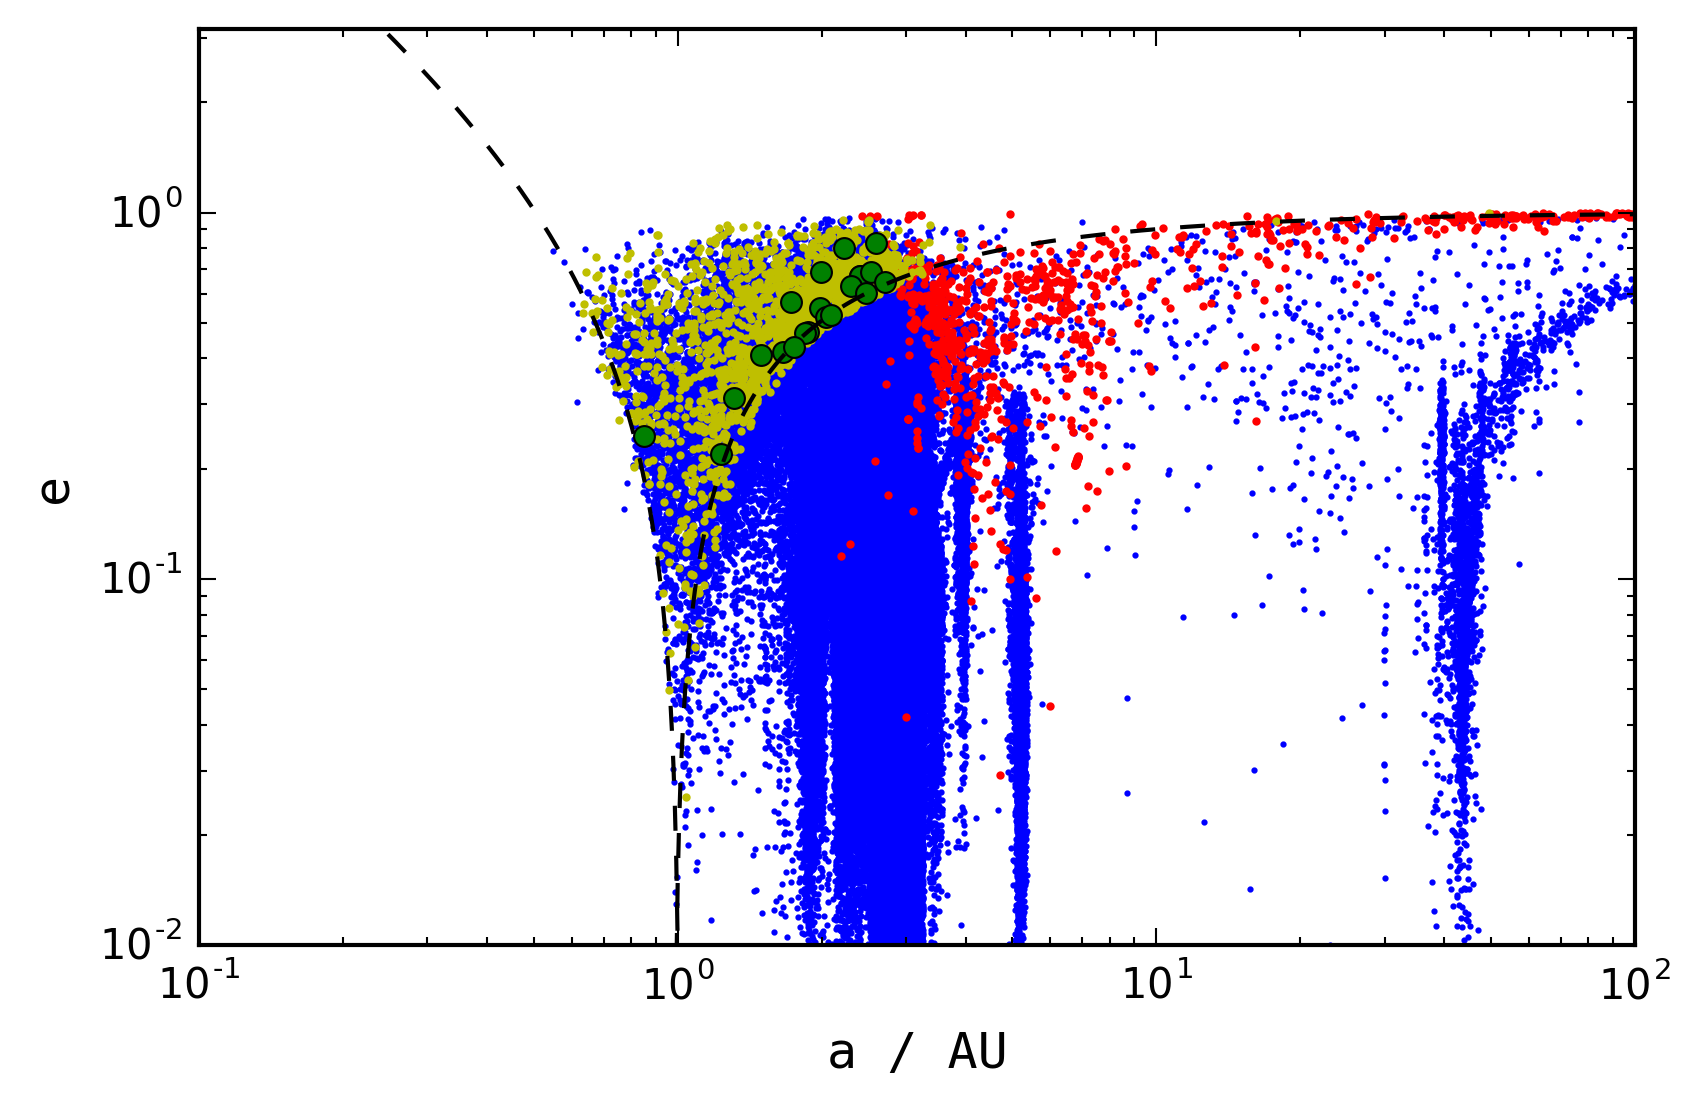
\includegraphics{losscone.png}
    \caption[Catalogued asteroids and comets in Earth's loss cone]{Semi-major axes vs eccentricities of observed asteroids (blue), comets (red) and potentially hazardous asteroids (yellow). Data sourced from the IAU MPC. Meteorites with pre-impact orbits determined by \cite{doi:10.1093/mnras/stv378} are plotted as green circles. The Earth aphelion and perihelion are plotted as dashed lines.}
    \label{fig:loss_cone}
\end{figure}

\begin{figure}[h!]
    \centering
    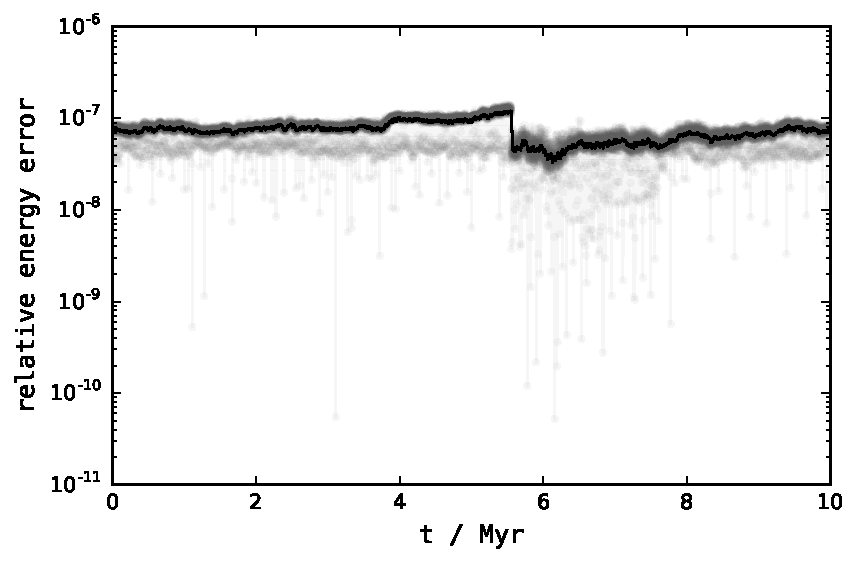
\includegraphics{figures/error.pdf}
    \caption[Simulation error]{Relative energy error over time. Black line shows the moving average of all the simulation runs.}
    \label{fig:error}
\end{figure}

%\section{Worst-case scenarios}

\begin{figure}[h!]
    \centering
    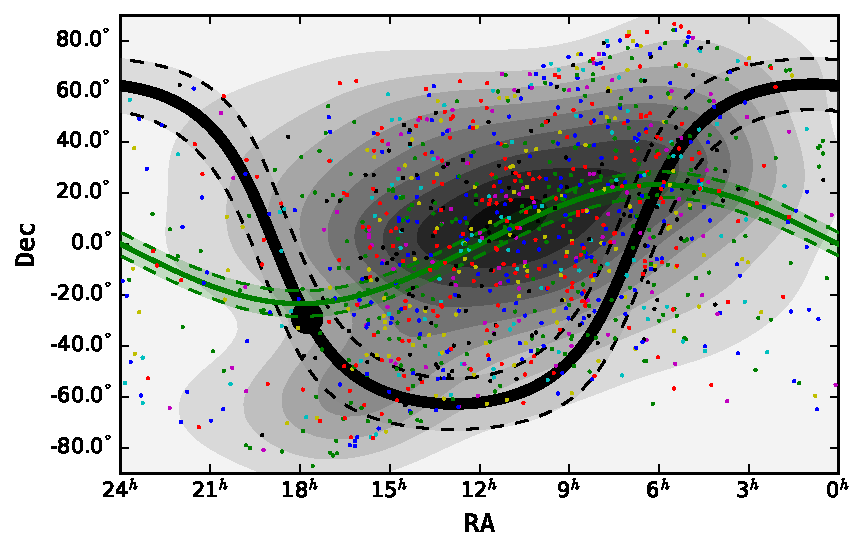
\includegraphics{radiants.pdf}
    \caption[Distribution of apparent radiants]{Distribution of apparent radiants for comets at the point of impact. Geocentric equatorial coordinates (J200) plotted for various comet threats. Comets that spent the majority of the simulation length in the JFC class are marked as triangles. Plus markers for HFCs, circles for centaurs, squares for TNOs and diamonds for Encke-type comets. Different marker colours denote separate simulation runs. Green line and boundaries represent the plane of the ecliptic $\pm5^\degree$, black line and boundaries represent the galactic plane $\pm10^\degree$. The galactic centre is plotted as a black circle. A 2D kernel density estimate is shown.}
    \label{fig:radiants}
\end{figure}

\begin{figure}[h!]
    \centering
    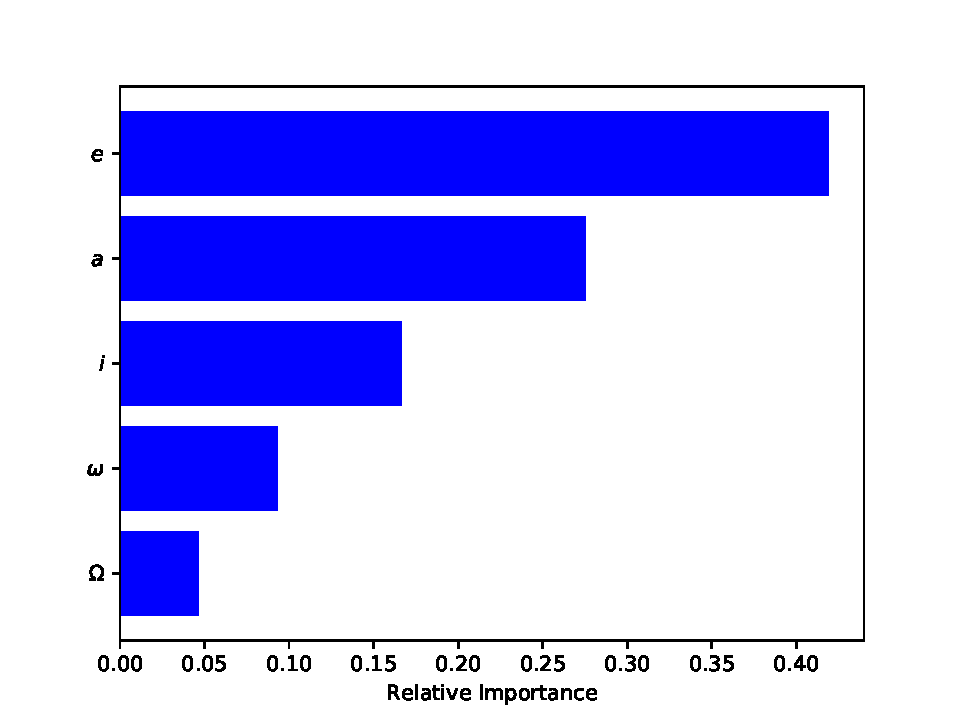
\includegraphics[width=\textwidth]{gini.pdf}
    \caption[Relative importance of orbital characteristics in learning algorithm]{Relative importance of each feature used for classification in the random forest learning algorithm. Gini importance calculated by examining the total reduction of $I_G$ due to a particular feature across all our decision trees.}
    \label{fig:gini}
\end{figure}


\begin{sidewaystable}[h!]
\caption[Initial conditions]{Initial conditions of the solar system as of 01-12-2017 12:00 UTC. Data sourced from NASA JPL Horizons database.}\vspace{3ex}
\label{table:init_con}
\begin{tabular}{llllllll} \toprule \toprule
\multicolumn{1}{c}{Object} & \multicolumn{1}{c}{Mass / $M_{\odot}$} & \multicolumn{1}{c}{$x$ / AU} & \multicolumn{1}{c}{$y$ / AU} & \multicolumn{1}{c}{$z$ / AU} & \multicolumn{1}{c}{$v_x$ / AU$\;$yr$^{-1}$}& \multicolumn{1}{c}{$v_y$  / AU$\;$yr$^{-1}$}& \multicolumn{1}{c}{$v_z$  / AU$\;$yr$^{-1}$}\\ \midrule
Sun & 1.000E+00 & 1.977E-03 & 5.974E-03 & -1.244E-04 & -2.047E-03 & 1.909E-03 & 4.906E-05 \\
Mercury & 1.660E-07 & 3.336E-01 & 8.143E-02 & -2.438E-02 & -4.270E+00 & 1.048E+01 & 1.248E+00 \\
Venus & 2.448E-06 & -4.901E-01 & -5.244E-01 & 2.100E-02 & 5.361E+00 & -5.058E+00 & -3.788E-01 \\
Earth-Moon system & 3.040E-06 & 3.515E-01 & 9.280E-01 & -1.647E-04 & -5.980E+00 & 2.206E+00 & -1.903E-05 \\
Mars & 3.227E-07 & -1.649E+00 & 3.172E-03 & 4.033E-02 & 1.975E-01 & -4.673E+00 & -1.028E-01 \\
Jupiter & 9.548E-04 & -4.396E+00 & -3.189E+00 & 1.115E-01 & 1.586E+00 & -2.100E+00 & -2.676E-02 \\
Saturn & 2.859E-04 & -1.129E-01 & -1.006E+01 & 1.793E-01 & 1.926E+00 & -2.944E-02 & -7.613E-02 \\
Uranus & 4.366E-05 & 1.778E+01 & 8.962E+00 & -1.970E-01 & -6.572E-01 & 1.216E+00 & 1.303E-02 \\
Neptune & 5.151E-05 & 2.865E+01 & -8.684E+00 & -4.815E-01 & 3.249E-01 & 1.104E+00 & -3.022E-02 \\
\bottomrule
\end{tabular}
\end{sidewaystable}

\clearpage
\section*{Derivation of $T_J$}

We first consider a system consisting of the point-masses of the Sun, Jupiter, and a comet. Each have a mass of $M_\odot$, $M_J$ and $M_C$ respectively. As $M_C \ll M_\odot$ and $M_C \ll M_J$, and the Sun and Jupiter have eccentricities very close to 0, one can describe the dynamical system in question as an example of the restricted three-body problem.

As $M_\odot \gg M_J$, the gravitational effect of Jupiter on a comet only becomes non-negligible in the event of a close encounter. As such, a comet exists in a standard elliptical orbit around the Sun with fixed orbital parameters that only change after a close approach.

The semi-latus rectum of the comet's orbit $p$ can be related to various other orbital parameters with,

\begin{equation}
    p = \dfrac{h^2}{GM_\odot} = a(1-e^2)~,
\end{equation}

where $h$ is the specific relative orbital angular momentum, $G$ the gravitational constant, $a$ the semi-major axis in units of Jupiter's semi-major axis $a_J$, and $e$ the orbital eccentricity.

The (approximately) conserved value of $h$ for the comet before and after its close approach to Jupiter can therefore be written as,

\begin{equation}
    h^2 = a(1-e^2)~.
\end{equation}

The only known conserved quantity for the circular restricted three-body problem is known as the Jacobi integral $C$ and is related to the conserved energy per unit mass $\epsilon$,

\begin{equation}
    \epsilon = \vec{\omega}\dot\vec{h} - \dfrac{C}{2}~,
    \label{eq:jacobi}
\end{equation}

where $\vec{h}$ is directed normal to the comet's orbital plane and $\vec{\omega}$ is directed in the $z$ direction, taken to be 1 in our system of units. Unlike in the two-body problem, $\epsilon$ and $h$ are not conserved separately and only $C$ is said to be a constant of the motion.

It follows that,

\begin{equation}
    \vec{\omega}\dot\vec{h} = \omega h \cos{i} = \sqrt{a(1-e^2}\cos{i},
    \label{eq:tiss_dot}
\end{equation}

where $i$ is the orbital inclination of the normal to the comet's orbital plane to Jupiter's orbital plane.

Taking the (approximately) conserved energy per unit mass of the comet before and after its close approach to Jupiter to be $\epsilon = -1/2a$, it follows from Eqns.~\eqref{eq:jacobi} and \eqref{eq:tiss_dot} that Equation.~\ref{eq:tiss_param} is quasi-constant before and after the close encounter with Jupiter (or any other major planet). 

\clearpage
\section*{Orbital energy changes at perihelion for LPCs}

First we consider a LPC's orbital velocity with the use of the vis-viva equation,

\begin{equation}
    v^2 = \mu \left( \dfrac{2}{r} - \dfrac{1}{a} \right)~,
    \label{eq:visviva}
\end{equation}

where $\mu=GM_\odot$ is the standard gravitational parameter, and $r$ is the heliocentric distance.

By considering the instant perturbation on the comet's orbit due to the gravity of the planets, the relationship between the change in orbital energy $\Delta(1/a)$ is related to the orbital velocity change $\Delta v$ and can be written as,

\begin{equation}
    \Delta(1/a) = -\dfrac{2v}{\mu} \Delta v.
\end{equation}

From Eqn.~\ref{eq:visviva}, $v$ scales inversely with $r$. This means that $| \Delta (1/a) |$ is maximised when $r$ is minimised (at perihelion).

\section*{Code}

All the \texttt{Python} code used throughout the course of this investigation can be viewed online at \url{https://github.com/Spiruel/L4_Project}.